\documentclass{article}

\usepackage{array}
\usepackage[rightcaption]{sidecap}
\usepackage{graphicx}
\graphicspath{ {./images/} }

\title{Meerkats File Synchronizer - Final Report}
\author{Made in GB}
\date{}

\begin{document}
\maketitle{}

\tableofcontents
\newpage

\section{Introduction}
Wee live in a dynamic and fast paced world where access to data is no longer limited to having access to a single device. Information is now available and accessible through one click and people are carrying small computers in their hands most of the time by having smart phone devices and are able to access their files from anywhere in the world. Additionally, enterprises use the cloud as a means for collaboration to increase their workforce productivity and to meet their customers’ requirements of having mobile access to products and services.

Digital age and user mobility have made data availability crucial not only for individuals but for business alike. Demands for having timely access to data and to ensure data accuracy and redundancy have increased dramatically and the need for technical solutions to meet these requirements has risen accordingly. The solution to reduce the time and efforts that are needed to manage data among different devices and in different locations is by using file synchronization software. File synchronization software is the process to ensuring that files in two or more locations are updated via certain rules (wikipedia). Additionally, it is used for backup and for mobile access to files.


\hfill \break
In this project, we are embarked on a new journey where we develop file synchronization software to provide secure and seamless synchronization solution to enable data management processes such as file creation, deletion, modification, distribution, redundancy and availability.

Our solution targets different kind of users and can be used in different sectors of the business world such as health organizations, educational entities, financial companies and much more. Company’s employees for instance, who work at separate locations can use it to access and distribute files. Individuals can utilize it to upload their holiday photos, for example, and to view them from their different devices (windows desktop and mobile).

It also, can be run on Windows desktops and Android mobile devices at the same time. We have chosen to name our software Meerkats, because the meerkats are one of the most collaborative animals in the world, and one of the main features for our software is collaboration.

\begin{figure}[h]
    \centering
    
\includegraphics[width=0.95\textwidth]{logo}
    \caption{Meerkats Logo}
    \label{fig:logo1}
\end{figure}

In this report, we provide complete information about the file synchronization software project. Detailing information about how we worked together as a team to develop our product, the strategies we used to ensure the delivery of reliable and efficient solution as well as information about the features and the configuration of the software itself I addition to our future plan.


\section{Review}
File synchronization softwares are popular and the most famous ones are Dropbox, GoogleDrive, One Drive and Box. We have reviewed these popular solutions. We found them all to provide the same basic features, as they allow users to access, share and synchronie data. Choosing the right synchronization software really depends on the user’s needs and expectations, as each solution has its advantages and disadvantages. We have focused on the file synchronization feature in each solution to understand how it works.

\subsection{GoogleDrive}
\textbf{Storage and Cost:}
Signing up for GoogleDrive provide users with 15GB of storage space for free. It can be increased up to 1TB for 10 USD a month. Google Drive lets users automatically copy files onto their different devices.


\hfill \break %keep this break
\textbf{File Synchronization:}
The solution is compatible with Windows, Mac, Android, iOS and it implements a sync folder mechanism, adding a “Google Drive” folder to the user's file-system when they install the desktop client (the client is called “Backup and Sync”). Any folder users drop in it gets sent off to the cloud, then onto other devices. The disadvantage of this process that it requires that files be stored both on the users’ hard drive and in the cloud to work, which is not useful if users want to free up their disk space. To address this concern, Google has introduced a new feature to allow users select specific folders to help in free up hard drive space. Users need to click on “preferences” button to open a window that will let them turn sync off for specific folders,(see figure1)
One point to mention about GoogleDrive is that it uploads and downloads the entire file all over again when a change is made, which takes time, but it is worth mentioning that google has multiple data centers around the world, which decreases both users computer’s distance to the cloud and server congestion at the same time.


\subsection{DropBox}
\textbf{Storage and Cost:}
Users who sign up to DropBox get 2GB of storage for free. This limited space is considered as a disadvantage of using DropBox, as users who want to get extra disk space, such as 100GB, need to get a paid subscription for 10 USD a month.


\hfill \break
\textbf{File Synchronization:}
DropBox can be installed on Windows, Mac, Linux, Android, iOS, Windows Phone, BlackBerry, Kindle Fire.As with GoogleDrive, DropBox uses a sync folder with a new feature called block-level sync.This feature allows users to manage selective files stored in the sync folder from the “preferences” tool accessible via the DropBox taskbar icon (on PC), (see figure2). This is very important functionality as it helps users to save their disk space and to better utilize it to store important documents that they want to access it and share it from anywhere.


\hfill \break

\subsection{Box}
\textbf{Cost and Storage}
Box for personal use offers free storage up to 10GB. Users can opt for more flexibility and storage space up to 100GB, which requires 10 USD per month.

\hfill \break
\textbf{File Synchronization}
Box applies the same file synchronization method invented by DropBox. Adding files and folders to the Box Sync folder on computer will automatically upload them to user’s account on Box.com and mark them for Sync. Users can selectively sync folders to better manage their disk space (see figure3). The solution can be run in Windows, Mac, Android, iOS, Windows Phone, BlackBerry.In 2018, Gartner assessed 14 Enterprise File Sync and Share (EFSS) and named Box as a leader in
2018 Magic Quadrant for Content Collaboration Platforms. (see  https://www.box.com/en-gb/resources/gartner-ccp-magic-quadrant)


\hfill \break
\subsection{OneDrive}
\textbf{Cost and Storage}
OneDrive is a Microsoft product and it offers up to 5GB free storage space. Users can pay 2 dollars a month to increase the storage size to 50GB. The solution is a great productivity tool since it is integrated with many other Microsoft products, such as Office Online, Skype, Outlook and the Office 365 suite for desktop.


\hfill \break
\textbf{File Synchronization}
OneDrive can run on Windows, Mac, Android, iOS, Windows Phone and it follows the standard sync model developed by DropBox. It includes a sync folder, which is like a normal folder with the only difference being that it’s connected to the cloud. OneDrive offers simple way to sync files. Users can move individual files to OneDrive’s sync folder by right-clicking and selecting “move to OneDrive”. A drawback about OneDrive is that specific files can’t be synced to OneDrive. Instead, users have to go to the settings menu of the OneDrive desktop client and update the folders (see figure 4) that OneDrive selected to “auto save” On Windows 10, they are “desktop,” “pictures” and “documents.” (seehttps://www.cloudwards.net/review/onedrive/)



The solution is compatible with Google docs and with some of office tools, which provides convenience for users who have google accounts as they can save their attachments directly into their googleDrive.(to be added if we needed more words later)
\newline
\hfill \break
We also looked at some resources such as Open Web Application Security Project (OWASP) to learn more about risks associated with web applications, secure software development, cloud and file security ''


\section{Requirements and design}
Project’s requirements have been supplied by the project’s supervisor (Dr. Laurance) for which the team has precisely aligned the software design, project timeline and allocated resources to meet the expectations.

\subsection{Project Deliverables}
By completing this project, the following deliverables are achieved.
\begin{enumerate}
  \item \textbf{File Storage Server} This component is used to store files and deal with requests received from users.
  \item \textbf{Mobile Client} It is an Android solution. Users can use the app on the go and will enjoy features such as Sign Up, Log In, View Files, Upload Files, Rename Files, Delete Files, etc.
  \item \textbf{Desktop GUI Client} The desktop GUI client is based on the Windows OS and it includes the same features as the mobile client.
  \item \textbf{Meerkats File Synchronizer Report} This report provides detailed information about the project in terms of team members, project plan, deliverables, timeline, technologies used, challenges and much more. It acts as a central reference for users who are interested in the software.
  \item \textbf{Meerkats File Synchronizer Presentation} The team will put together slides to present the work done. The team will demonstrate the solution and its layout, features and will walk the audience through the function- alities supplied by the software.
\end{enumerate}


\subsection{Business Requirements}
POSSIBLY MERGE THIS WITH DELIVERABLES
ADD SOME SORT OF INTRO HERE
\begin{enumerate}
  \item Develop File Synchronization Software
  Description:  File synchronization software is used to store copies of files to another device or to the cloud. The files are typically available to be accessed via a Web-based portal. Some examples of file sync software include Box and Dropbox.
  \item Build a ‘hub and spoke‘ file synchronizer
  Description: File synchronizer will allow communication between a single central server (the ‘hub’) to which multiple other clients (the ‘spokes’) synchronize.
  \item Develop a web server and two clients (desktop, mobile)
  Description: A web server will be developed and it will exchange data with mobile client (Android) and desktop client (Windows)
\end{enumerate}


\subsection{Project plan}

\begin{figure}[h]
    \centering
    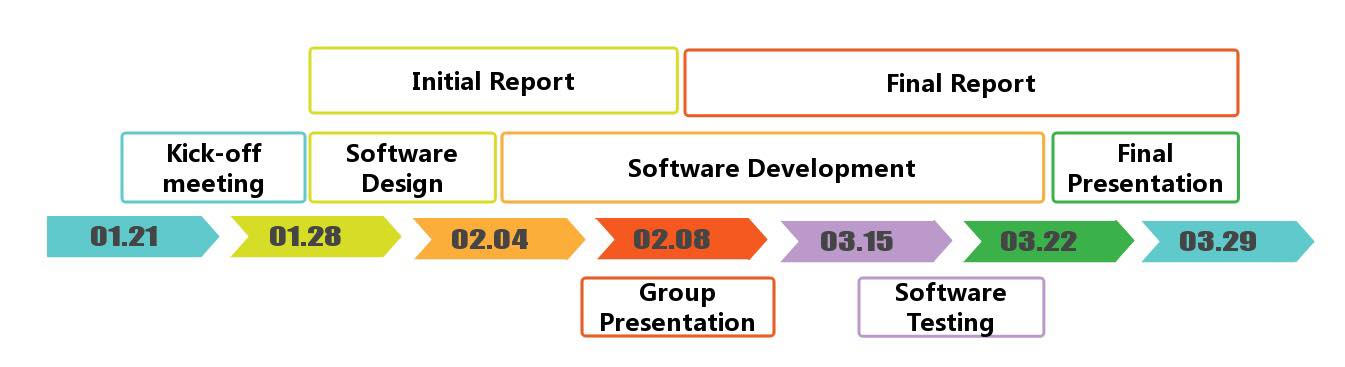
\includegraphics[width=1\textwidth]{timeline}
    \caption{Timeline}
    \label{fig:timeline1}
\end{figure}

TALK ABOUT TIMELINE.

\subsection{Implementation Timeframe}
Below table outlines the milestones along with brief description and expected timeframe.

\begin{center}
\begin{tabular}{ | m{3em} | m{2cm}| m{3cm} | m{1cm} | m{1cm} | m{2cm} |}
\hline
\textbf{\#} & \textbf{Milestones} & \textbf{Description} & \textbf{Start Date} & \textbf{End Date} & \textbf{Status}  \\
\hline
1 & Kick-off meeting & Background survey and initial plan & Jan 21, 2019 & Jan 27, 2019 & Completed \\
\hline
2 & Software Design  & Design the software layout & Jan 28, 2019 & Feb 3, 2019 & Completed \\
\hline
3 & Software Development & Work to deliver the file synchronization software & Feb 4, 2019 & March 21, 2019 & Completed \\
\hline
4 & Initial Report & To develop and submit the initial report & Jan 29, 2019 & Feb 7, 2019 & Completed \\
\hline
5 & Group Presentation & To demonstrate  the group initial software design and share the project plan & Feb 8, 2019 & Feb 8, 2019 & Completed \\
\hline
6 & Software Testing &  To test the software and ensure correct and secured implementation & March 15, 2019 & March 21, 2019 & Completed \\
\hline
7 & Final report & To submit the final report describing complete information about the software and the project lifecycle & Feb 8, 2019 & March 28, 2019 & Completed \\
\hline
8 & Final Presentation & To deliver the final presentation about the software & March 22, 2019 & March 29, 2019 & In progress \\
\hline
\end{tabular}
\end{center}

\subsection{Design Model}
The team has decided to follow the strategy of capitalizing on existing experiences and skills to save time and to deliver efficient solution.Some of the team members had the opportunity to develop android applications and others had the chance to build windows applications. Therefore, it was wise to go with those platforms since the expertise exists in the group in addition; those systems are reliable and widely used by users.

The following flow charts show the general design of the solution as well as detailed design for the Android and Windows clients.

\begin{figure}[h]
    \centering
    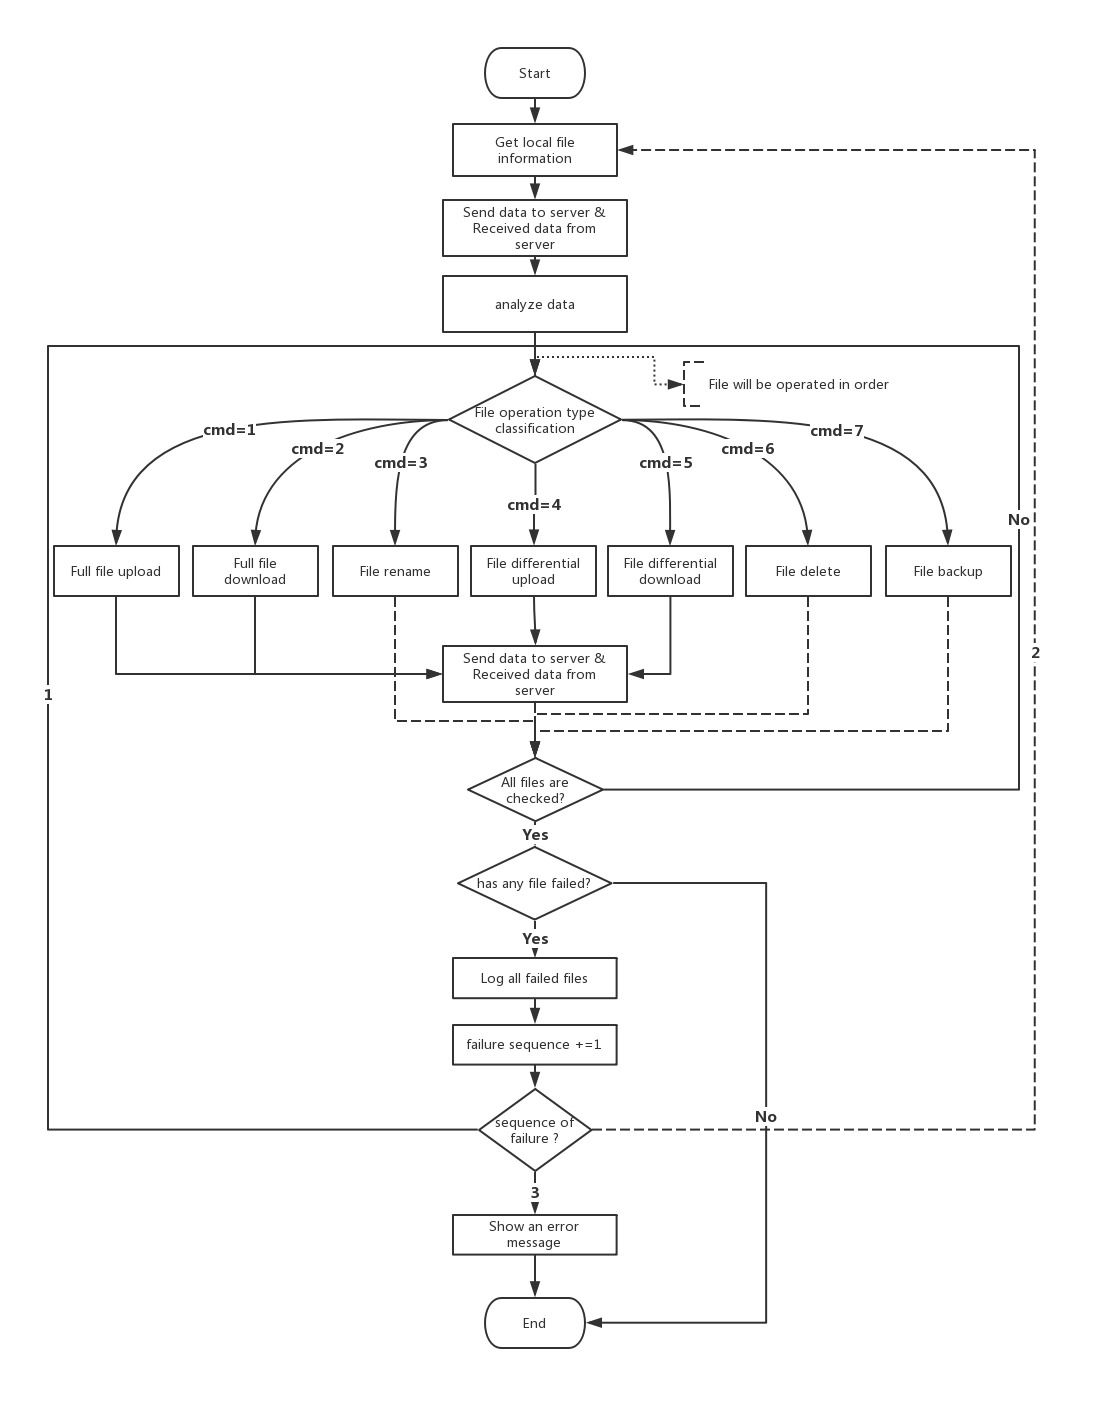
\includegraphics[width=0.95\textwidth]{flowchart}
    \caption{Flowchart}
    \label{fig:flowchart1}
\end{figure}


This diagram shown in Figure 3 shows two main functions of the file synchronization software that are executed through desktop application.
The flowchart illustrates how the upload and download functions are implemented in details, from the time a user clicks on upload/download till complete execution of those requests.

\subsection{Mobile Application Interface Design Principles}
We understand that designing mobile application is very different than designing desktop application.
Therefore, we have got into mobile design mindset before starting designing the mobile app.
We designed the mobile client interface with great intent to impress users within the few seconds after they start using it and to retain them in the long run. We tried our best to create an excellent User Experience (UX). For that, we have searched the Internet and learned about UX and how it contributes to the success of any new application. We also spent much time in searching and looking for a variety of design examples for inspirations. We have come up with intuitive and creative mobile interface design where we have followed collection of interface design principles that include but not limited to:

\begin{enumerate}
\item \textbf{Consistency of the design layout:} We made sure to design the sections of the application to be coherent, and we provided a consistent flow of the layout throughout the app.
\item \textbf{Unambiguous Interactive Elements:} Elements that are intended for interaction with users are clearly depicted. Key options such as Create, Delete and Rename are visible and easy to access by users when required by them without the need to search for hidden options in menus.
\item \textbf{Single Trial Learning Experience:}  Since we aim to create user friendly application, we designed the app and placed the options tin a way that allow users to anticipate the next step and the flow of the process in general without the need to remember the steps.
\item \textbf{Layered User Experience:} We understand that UX should be layered. Meaning that not all the features and options of the app are visible at once. We kept some buttons hidden as we wanted to keep the interest of users for longer time and as they go deeper into the app. However, we balanced between keeping the excitement of users and the simplicity of navigating the app.
\item \textbf{Navigation Models:} We know that there are many navigation models out there but we chose tab bar or Drill down because it makes the most sense of our application.
\item \textbf{Orientation:} Is how the keyboard looks like when users attempt to type in their data. We have selected Portrait as our application doesn’t require lots of data to be inputted.
\item \textbf{Launching:} When users launch the application, they will see an image that represent the logo of the software and the application name only. We aimed at not to confuse users at the beginning by adding buttons and text when they firs load the application. When users leave the app and comeback to it, they will resume operation right where they left the application.
\item \textbf{First impressions:} We believe on the say “ first launch make or break situation” therefore, we though of the following things:
\end{enumerate}
\begin{itemize}
\item \textbf{Icons:} We have kept text to minimum, and selected polished and eye attraction icons to attract users attention and create excellent and lasting first impression.
\item \textbf{First launch:} We ensured that users are not lost when they first launch the application and can easily deal with it without the need to seek assistance.
\end{itemize}

\begin{figure}[h]
    \centering
    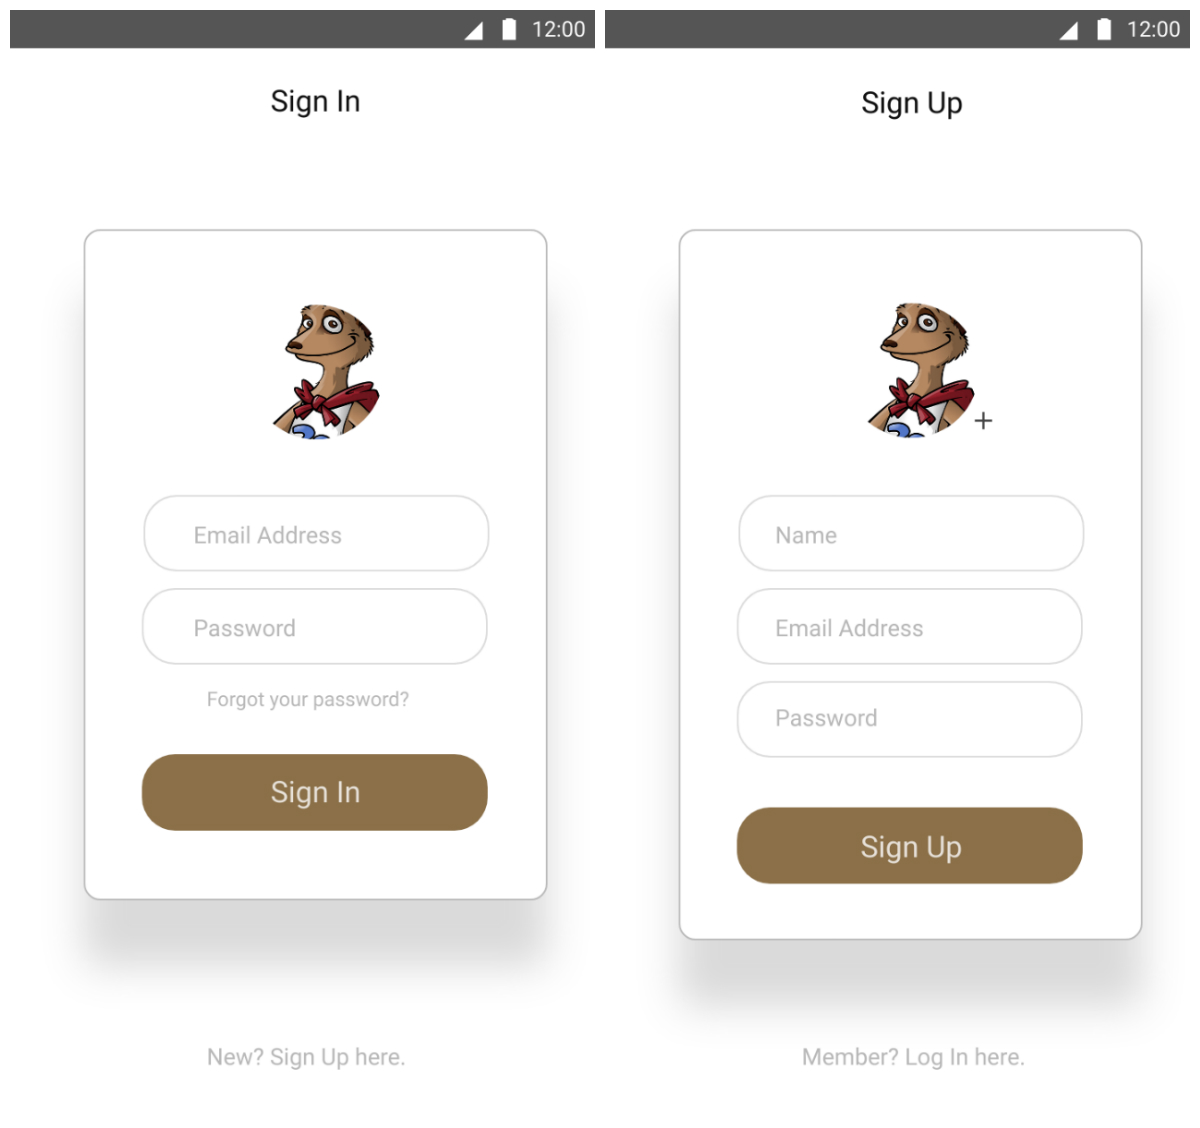
\includegraphics[width=0.95\textwidth]{signup}
    \caption{Sign in and sign up screen}
    \label{fig:signup1}
\end{figure}

\subsection{Desktop Application Interface Design Principles}
As with mobile app interface design interface, our goal was to create a perfect user experience. We thoroughly thought of how to design desktop application interface that is simple to use, fun to interact with and intuitive. Some rules that we considered include the following:
\begin{itemize}
\item Combine what should be combined. Features that support the execution of a task have been gathered in one place. Consequently, tasks that are performed through multiple steps can be performed in streamlined flow.
\item Separate what should be separated. To support simplicity and avoid complex interface, key features are presented in very clear way while optional and secondary features are hidden. We also, separated tasks related to specific function (creation of a new file for example) from tasks supporting another function (uploading existing file).
\item Eliminate what can be eliminated. The interface design has been reviewed to examine the text and all elements to make sure that clear, simple and easy to understand words are used and no redundancy in the element.
\item Put the elements in the right place. We followed logical order when placing buttons and instructions. Progressive Disclosure Technique has been considered as applicable. It is about displaying additional information as needed instead of filing the home page with too many elements and information.
\item Use meaningful high-level combinations. It is often simpler and more scalable to select and manipulate groups of related elements than individual elements. Examples of high-level combinations include folders, themes, styles, and user groups. Such combinations often map to a user goal or intention that isn't apparent from the individual elements. For example, the intention behind the High Contrast Black color scheme is far more apparent than that of a black window background.
\item Select the right controls. Design elements have presented in efficient manner by selecting the right controls. We know that selecting the right controls are important to effectively interact with the application. For example, the saving file function has been presented in a simple dialog box that ask the users to enter the file name and type then have the options to save it or cancel the transaction.
\end{itemize}


\subsection{Security Design}

The team worked hard to ensure not only delivering functional solution but also a secured product. For that, the team followed the security principles that were cited in OWASP Development Guide. They include:

\begin{enumerate}
\item \textbf{Minimise attack surface area??}
We tried to minimize the attack surface area by producing file synchronization software that is capable to perform essential functions that users are interested in  such as create, delete, rename and modify files to reduce potential threats and the possibility of exploiting vulnerabilities in the application.
For example, we coded file search feature into the application. That search feature is potentially vulnerable to SQL injection attacks. But we have developed data sanitization control to prevent users from sending sql injection directly to the file server and by doing so, we are reducing the attack surface and success attempts to manipulate data.
\item \textbf{Establish secure defaults}
The solution was designed to be secure by default. On another word, we have disabled some privileges for non-admin users and activated other security features by default to enhance the security status of the application and reduce the likelihood of attacking the application. For example, when creating new file, users are not allowed to use special characters in the file name, absolute file path is not allowed as well as file names that could be misinterpreted by the server is prohibited.
\item \textbf{The principle of least privilege}
The Principle of Least Privilege (POLP) has been applied to all aspects of the application. The team has designed the solution in away that allows users to execute tasks with minimum privileges required to perform that task.
For example,
\item \textbf{The principle of Defense in depth}
The principle of defense in depth is considered in the design. The team used different security controls to approach different risks such as data leakage, data unavailability, code injection…etc.
\begin{itemize}
\item \textbf{Process Title:} Establishing Secure Connection (Handshake)
\item \textbf{Risk:} Adversaries could intercept the connection between the client and the server and/or alter data or view sensitive data, in addition to repudiation risk.
\item \textbf{Security Control Title:} Rivest-Shamir-Adleman (RSA) Algorithm. RSA was used to provide secure connection and protection of data storage. The security of an algorithm depends on the length of the private key and since it is so far very difficult for attackers to compute large prime number, which is the result of multiplying two large primes we selected RSA.

\item \textbf{Process Title:} Key Exchange Stage through (Diffe-Hellman) Algorithm
\item \textbf{Risk:} Private keys can be accessed by unauthorized people, which could result in their ability to decrypt cipher text and get access to sensitive data in plaintext.
\item \textbf{Security Control:} Since we used RSA to encrypt the connection, it is very important to use secure method to exchange keys. We used Diffe-Hellman because it is a simple yet secured algorithm to facilitate key exchange.

\item \textbf{Process Title:} Data Stream Encryption through Advanced Encryption Standard (AES)
\item \textbf{Risk:} Data travel over the internet in plaintext format are vulnerable to many threats such as unauthorized access and potentially malicious modification by adversaries. To protect against those threats, we used AES to encrypt the communication between the server and the clients.
\item \textbf{Security Control:} Data Stream Cipher- Advanced Encryption Standards (AES). This cipher was used to encrypt data when they are streamed to the cloud.

\item \textbf{Process Title:} Securely Transmitting and Synchronizing Files
\item \textbf{Risk:} The integrity of files transferred over the Internet and stored in the web need to be protected from unauthorized modification and data manipulation.
\item \textbf{Security Control:} We are using a cryptographic hashing function ‘Message Digest (MD5) ‘ to validate data integrity when digitally transferred over the Internet. MD5 produces 128-bit hash value to check data integrity. We selected MD5 as it is simple to be implemented and we are considering using more secure non-cryptographic hash function such as MurMur in future since it has less structure considering the number of assembly instructions it generates as well as it provides a better collisions resistance than MD5.

\item \textbf{Process Title:} File Upload
\item \textbf{Risk:} Uploading infected or malicious files.
\item \textbf{Security Controls:} Using Anti-Virus program to scan files before they are uploaded to the cloud.
\end{itemize}

\item \textbf{Fail securely}
The application was designed to fail securely. That means, even if a failure occurs, it won’t expose sensitive data like logs or grant users additional privileges.
\item \textbf{Avoid security by obscurity}
Security controls are in place to protect the application core functionalities and codes without necessary the need to rely on security by obscurity.
\item \textbf{Keep security simple}
We have avoided the use of complex design when developing security controls for the software. Instead, we made sure to use simple yet efficient security controls to reduce security errors.
\item \textbf{Fix security issues correctly}
The team address security issues that have been identified during the testing phase by determining the root causes of the problems. They are then repair it and test the repairs thoroughly.
\end{enumerate}

\section{Implementation}
The team has spent great deal of time searching and deciding on the best approach to execute the project and the right methodology to develop the building blocks of the software and the integration among those components.

\subsection{Development Guiding Principles}

\begin{itemize}
  \item Simplicity (Say something about each item maybe??)
  \item Previous experience
  \item Efficiency
  \item Speed of execution
\end{itemize}


\hfill \break
\textbf{Programming languages}
We discussed among the team what are the right languages to use to develop the server, mobile client and desktop app and we agreed on the following languages:
\begin{itemize}
\item\textbf{The Server:} The group decided to use Golang knows also as Go for building the server. Golang is an open source programming language that makes it easy to build simple, reliable, and efficient software. Go has great advantages such as no pointer arithmetic, no manual memory management, a standard library that seems fairly well thought out and purposefully excludes things that are misused (ex. no ECB mode for AES).
\item\textbf{The Mobile Client:} Java was used to build the android mobile application. The reason for choosing Java is it is a commonly used language and some of the team members know it very well.
Additionally, many development tools are available for Java. It is a popular object oriented programming language with most phones compatible with it.
\item\textbf{The Desktop Client:} C Sharp was selected to build windows desktop application because it is targeted toward windows operating system. Some team members had the chance to use it and have the skills to develop desktop application using C sharp. Additionally, C sharp has a built-in advanced code editor and debugger, which leads to debugging errors in quicker manner. It also, has an intensive framework, which make
\end{itemize}

\hfill \break
\textbf{Data Storage and Transmissions Method}
Serialization was used to enable data transmission between the devices. In computer science, in the context of data storage and transmission, serialization is the process of converting a data structure or object into a sequence of bits so that it can be stored in a file or memory buffer, or transmitted across a network connection link to be "resurrected" later in the same or another computer environment. (Wikipedia). There are two ways of transmitting data between server and browser and in which we can encode data. The two methods are JavaScript Object Notation
(JSON) and Protocol Buffers known as Protobuf. We decided to use JSON as it meets our technical needs and for simplicity and convenience. JSON uses Ajax to enable the exchange of data between the web application and the browser and server without the need to reload the page and it encodes data in a human readable manner. However, in future version of the software, we might switch to Protobuf to overcome some limitations in JSON such as the slowness of encoding and decoding for integers and floats, comparing strings is a bit time consuming as well as the need for sequential scan when parsing strings, arrays and objects which in all preceding cases are mitigated in Protobuf.

\hfill \break
\textbf{Communication Protocol}
The software is running over the TCP protocol through the xxxx(???) port. The team originally have thought of two protocols that are TCP and HTTP. We decided to use TCP due to its simple structure and easy to follow and implement rules
\newline
\hfill \break
\textbf{Rsync: An overview:} We have looked at Rsync as suggested by the project supervisor and found it to be sufficient to do the job. In a nutshell, Rsync is used to detect changes in files that are stored in two different locations and then sync the file in the remote sever to be identical to the file that is stored in local hard drive without the need to send the complete file over the internet to the server once again each time a user makes a change in the local version of it.
\newline
\hfill \break
\textbf{How it works:}
Below steps were copied from \underline{jenkov.com} as they well describe how rsync works.
\begin{enumerate}
\item The computer holding the newest version of the file is here called NEW, and the computer holding the oldest file is called OLD.
\item OLD divides the oldest version of the file into blocks of, say 1024 or 2048 bytes. The file is not divided on the disk. It's just something OLD does logically, internally in the memory.
\item For each block OLD calculates a checksum.
\item The list of block checksums are sent to NEW.
\item NEW searches the newest version of the file for blocks of data that has the same checksum as those found in the old version of the file. This is done by fist calculating the checsum for the very first block of data (1024 or 2048 bytes). If this checksum does not match any checksum in the old file, NEW moves 1 byte down the new file and calculates the checsum for this 1024 checksum. NEW thus calculates checksums for every possible 1024 (or 2048) byte block in the new file, to search for matches to blocks in the old file.
\item If NEW finds a 1024 byte block with the same checksum as one of the checksums received from OLD, then it considers that block to exist in the old version. It doesn't matter if the sequence of blocks is not the same as in the old version. NEW now skips to the end of this block and continues searching for checksum matches from there.
\item NEW will thus find X blocks of data matching checksums in the old file. This is the data that has not changed between the old and the new version of the file. In between these blocks will be data that was not part of a 1024 block that matched a checksum in the old file. This data is CHANGES, either new or modified data.
\item NEW sends back instructions to OLD on how to create a copy of the newest version of the file. NEW does this by sending a list of block references in the old file for the sections of the newest file that has not changed. For the parts that has changed NEW sends back the changed data in full.
\item OLD receives the list of block references and literal data (the changes), and from the old file and the literal data, constructs the new version of the file.
\end{enumerate}
\textbf{User Interface Testing}
The team spent some time doing usability testing to check the user experience before completing the deployment of the software. Usability testing aimed at verifying that using the application is going to be a perfect user experience and users will live an enjoyable experience when interacting with the services provided by Meerkats.
\newline
\hfill \break
\textbf{Functionality Testing}
\newline
\hfill \break
\textbf{Connectivity Testing}
\newline
\hfill \break
\textbf{Security Testing}


\section{Team work}
Our team strongly believes on the principle "The whole is greater than the sum of its parts". The team consists of six students, and throughout the project lifecycle, we tried to tap into each individuals strength, and challenge each other to gain new knowledge. We aimed to make this expedience as enjoyable, yet beneficial, as possible.

\subsection{Effective Communication}
When we first got together, we discussed the importance of setting communication ground rules. We all come from different backgrounds and are used to different cultures. For that purpose, we developed "Communication Ground Rules", of which the team agreed to fully abide by those rules. The rules aimed to reduce the possibility of misunderstanding, conflicts and to ensure commitment and respect among the team.

Here are the group’s communication ground rules:
\begin{enumerate}
  \item Mutually commit to our team’s objectives as stated in the project report or negotiate until we can make this mutual commitment.
  \item All team members are expected to attend team meetings unless they are out of town or sick. If a team member is unavailable, he or she should notify the rest of the team and should share their update through email or Skype.
  \item Team meetings will start and end on time.
  \item Action items will be distributed within 24 hours after the meeting.
  \item Understand each other’s styles.
  \item Tackle issues, not people.
  \item Permit one speaker at a time (avoid side conversations).
  \item Bring issues to the table during the team update meeting.
  \item Explain the reasoning leading to your conclusions.
  \item Invite inquiry into your views.
  \item Inquire into the reasoning of others.
\end{enumerate}


Furthermore, the team depended on Google Docs to share links and important updates, and GIT to store project documentations. We also utilized technology such as Slack to facilitate instant conversation and to share information about the project, which has significantly saved everyone’s time.

\subsection{Conflict Management}
The team members were inspired to provide a friendly project environment that enabled everyone to put in their best efforts. We aimed to build a resilient team that responded to challenges, unforeseen events and different circumstances in a timely manner.

One way to avoid conflict was to use consensus for important decisions and issues. For less important issues, we relied on the subject matter expert with input from others. This approach worked well throughout the entire project.


\hfill \break %dont remove this line for some reason
The team also considered this group project as an opprotuenty to build the following types of skills:


\begin{itemize}
\item \textbf{Communication Skills:} Good communication skills are the most basic skills that one can possess as an employee or student. We aim to improve the team members ability to communicate effectively with each others and to convey information in a simple and unambiguous way.
\item \textbf{Practice Diversity:} The team consists of 6 members who come from different countries, speak different languages and have different backgrounds. We aim to learn how to recognize individual differences and understand how cultural differences can impact how people work, and interact.
\item \textbf{Project Management Skills:} Take this project as an opportunity to build project management skills that are essential to successfully complete a project that includes but not limited to planning, leadership, communication, and risk management.
\item \textbf{Teamwork Skills:} Teamwork is important for the success of this project. We aim to build teamwork skills, which are essentials at work after graduation. Each member will learn how to be a good team player by demonstrating skills such as negotiation, communication, problem solving and prioritization.
\end{itemize}

\section{Evaluation}

\section{Peer assessment}
The team agreed to distribute the 100 score by each one equally as showing in the following table. The rational behind this decision is due to great efforts been put by everyone and as a reward for the continues commitment and hard work.


\begin{center}
\begin{tabular}{ | m{3cm}| m{1.3cm} | }
\hline
\textbf{Name} & \textbf{Points}  \\
\hline
Boyang Zhang & 16.66  \\
\hline
Xi He & 16.66  \\
\hline
YiFeng Zheng & 16.66 \\
\hline
Yenan Huang & 16.66 \\
\hline
Frida Solheim & 16.66 \\
\hline
Samah Alghamdi & 16.66 \\
\hline
\end{tabular}
\end{center}


\section{Challenges}
\begin{itemize}
\item \textbf{Communication:} Since we came from different background and since we speak different languages (Arabic, Chinese and Norwegian), having the ability to speak English clearly and be able to deliver information and updates in clear manner is vital to the success of the group. Our chines colleagues had a problem with demonstrating the ability to which resulted sometimes in miscommunication or \textbf{Solution:} We agreed to use very simple English words and terms when we discuss project update or argue ideas and that every one should ensure that his/her message has been delivered to every one correctly by using assurance questions such as am I clear? Did you understand my point? do you want me to repeat what I just said?...etc.

\item \textbf{Attendance Punctuality} In addition to our daily chats through slack, we decided to meet in person once every week to discuss progress, issues and better connect with each other’s. However, we had to cancel some meetings due to either tardiness of last minute notice of absence by some of the team members.
\textbf{Solution:} We created a process to address this issue. We agreed to deduct points from the peer-to-peer assessment scores if a member was late for more than 5 minutes of the meeting start time or didn’t inform the group about his/her absence 24 hours prior the meeting date.
This process ensured timely attendance and commitment of all team members.
\item \textbf{Project timeframe:}
Description

\item \textbf{Resources:}
Description
\item \textbf{Creating simple and user friendly interface:}
Description
\end{itemize}

\section{Future Work}
\begin{itemize}

\item \textbf{Design iPhone client}

\textbf{Description:} In addition for the software to be compatible with Windows and Android, we are planning to further enhance its usability by developing MAC client.

\textbf{Added Value:} More users especially those who have iphones and mac desktops are expected to use the software and benefit from its services.
\item \textbf{Introduce file versioning feature}

\textbf{Description:} File versioning feature enables archiving the old version of a file when users attempt to delete it or replace it with a newer version and still want to keep the old versions of the original file. This feature will be configured per file and on per-device fashion and it is usually defaulted to no file versioning are used.
We will decide on the file versioning strategies and will be using one of the available options such as automatically delete files if they are older than the maximum age or exceed the number of files allowed in an interval (one hour, one day, 30 days). Another strategy is to delegate file versioning method to an external program after specifying the versioning strategies.

\textbf{Added Value:} Since dealing with electronic documents involved rapid changes, there is a need to keep old versions to restore deleted files or undo certain changes. It will also, increase collaboration among team members who might be working on the same project as each person will have the chance to work on the same file at the same time and all versions will be kept in one repository.

\item \textbf{Offer paid subscription with premium features}

\textbf{Description:} We are thinking to offer specific features on paid basis since they will require special development and allocation of resources. We are planning to offer greater storage capacity, longer file versioning duration to premium users

\textbf{Added Value:} To increase the customer satisfaction by introducing new features that help to increase their productivity and make the software more responsive to customers’ needs such as the desire to have larger storage space.

\item \textbf{Anticipate and Answer Users’ Queries:}

\textbf{Description:} When users tap a button, they want to know whether the process has started and how long will it take. As technology abstracts these actions, the users are usually kept in the dark while the process is going on. Use Toast in Android and notifications in iOS so users will be notified when a process has completed. The Gmail app is a good example of such a design, as it displays messages like “saved in draft, message sent, etc.” to inform the users about the completion of the task.

\textbf{Added Value:} better user experience as users can anticipate how long it will take to complete their request and better manage their times.
\end{itemize}

\section{Things I am adding later/working on}
DONT MIND THE FORMAT??

Finite-State Matchine(FSM)
What is a FSM?
Our server implements a FSM model to process incoming TCP stream of bytes.
You can find out what my implementation is in the part of “Pseudocode For Depacking”. (http://t.cn/EIi6Kxs)

Serialization Method Comparison (JSON vs Protobuf)
What are the two method?
What are their features?
Protobuf is a more advanced method, but we use JSON as our encoding method for simplicity and convenience. We can still mention in the “lessons we got” or “our future work” part of our final report that we will involve Protobuf in our next version.

Hash Functions (Comparison)
We adopt md5 also for simplicity. algorithm?
What is its mechanism?
Make a comparison between common algorithms. Specially, a newly developed algorithm called MurmurHash should be considered. Also, you can put it to “our future work” part.

Compression Method(gzip)
What is gizp?
Gzip is both a file format and a software application that is used for file compression and decompression.
What is its mechanism?


Our Security Mechanism
Hopefully we can achieve it after developing all the basic functions!
Shake-hands Stage(RSA)
Key Exchange Stage(Diffe-Hellman)
Data Stream Encryption Stage(industrial-level algorithms:AES or RC4, features?performance?make a comparison)

Git Feature Branch Workflow
We are using it now. What is it?What is its strength?

?
\end{document}
